\rfcnumber{0009}
\rfctitle{Session Start Protocol}
\rfcdate{October 2025}
\rfcauthor{Tino Breddin (@tolbrino), Lukas Pohanka (@NumberFour8)}
\section{RFC-0009: Session Start
Protocol}\label{rfc-0009-session-start-protocol}

\begin{itemize}
\tightlist
\item
  \textbf{RFC Number:} 0009
\item
  \textbf{Title:} Session Start Protocol
\item
  \textbf{Status:} Finalised
\item
  \textbf{Author(s):} Tino Breddin (@tolbrino), Lukas Pohanka
  (@NumberFour8)
\item
  \textbf{Created:} 2025-08-20
\item
  \textbf{Updated:} 2025-10-27
\item
  \textbf{Version:} v1.0.0 (Finalised)
\item
  \textbf{Supersedes:} none
\item
  \textbf{Related Links:}
  \href{../RFC-0002-mixnet-keywords/0002-mixnet-keywords.md}{RFC-0002},
  \href{../RFC-0004-hopr-packet-protocol/0004-hopr-packet-protocol.md}{RFC-0004},
  \href{../RFC-0008-session-protocol/0008-session-protocol.md}{RFC-0008},
  \href{../RFC-0011-application-protocol/0011-application-protocol.md}{RFC-0011}
\end{itemize}

\subsection{1. Abstract}\label{abstract}

This RFC specifies the HOPR session start protocol, which provides a
handshake mechanism for establishing communication sessions between
peers in the HOPR mixnet. The protocol manages session establishment,
lifecycle management, and capability negotiation, using HOPR packets as
the underlying transport layer. It defines a standardised method for
initiating sessions, exchanging session parameters (identifiers,
targets, and capabilities), and maintaining session state through
periodic keep-alive messages.

The session start protocol operates independently of the session data
protocol
(\href{../RFC-0008-session-protocol/0008-session-protocol.md}{RFC-0008}),
which handles actual data transmission once a session has been
established. This separation allows the handshake mechanism to evolve
independently from data transfer protocols.

\subsection{2. Motivation}\label{motivation}

The HOPR mixnet requires a standardised mechanism for establishing
communication sessions between nodes. While the session data protocol
(\href{../RFC-0008-session-protocol/0008-session-protocol.md}{RFC-0008})
handles reliable and unreliable data transmission, a complementary
protocol is needed for session initialisation. The session start
protocol addresses the following requirements:

\begin{enumerate}
\def\labelenumi{\arabic{enumi}.}
\item
  \textbf{Session establishment}: Provide a handshake mechanism to
  initiate sessions with capability negotiation, allowing peers to agree
  on session parameters before data exchange begins.
\item
  \textbf{Session identification}: Enable exchange of unique session
  identifiers and target endpoints, ensuring both peers can correctly
  route subsequent messages.
\item
  \textbf{Lifecycle management}: Define clear state transitions for
  session establishment, including timeout handling and graceful error
  reporting.
\item
  \textbf{Error handling}: Provide structured error reporting for common
  failure scenarios (e.g., resource exhaustion, busy nodes), enabling
  intelligent retry logic.
\item
  \textbf{Liveness maintenance}: Support keep-alive mechanisms to
  maintain long-lived sessions and detect peer failures.
\end{enumerate}

The session start protocol is intentionally lightweight and
transport-agnostic, making it suitable for use over various packet-based
transports while being optimised for the HOPR mixnet.

\subsection{3. Terminology}\label{terminology}

The keywords ``MUST'', ``MUST NOT'', ``REQUIRED'', ``SHALL'', ``SHALL
NOT'', ``SHOULD'', ``SHOULD NOT'', ``RECOMMENDED'', ``MAY'', and
``OPTIONAL'' in this document are to be interpreted as described in
{[}01{]} when, and only when, they appear in all capitals, as shown
here.

All terminology used in this document, including general mix network
concepts and HOPR-specific definitions, is provided in
\href{../RFC-0002-mixnet-keywords/0002-mixnet-keywords.md}{RFC-0002}.
That document serves as the authoritative reference for the terminology
and conventions adopted across the HOPR RFC series. 

Additionally, this document defines the following session start protocol-specific 
terms:

\begin{itemize}
\item
  \textbf{challenge}: A 64-bit random value used to correlate requests
  and responses in the handshake process. Challenge values MUST be
  generated using a cryptographically secure pseudo-random number
  generator (CSPRNG) and are interpreted as big-endian unsigned
  integers.
\item
  \textbf{session target}: The destination or purpose of a session,
  typically representing an address or service identifier. Session
  targets are encoded using CBOR format {[}02{]} to allow flexible
  representation of various endpoint types (e.g., IPv4/IPv6 addresses
  with ports, service URIs).
\item
  \textbf{session capabilities}: A bitmap of session features and
  options negotiated during session establishment. The capabilities
  field enables peers to agree on optional protocol features, with
  unrecognised bits being safely ignored to support backward
  compatibility.
\item
  \textbf{session ID}: A unique identifier assigned by the responder to
  identify an established session. Session IDs are encoded using CBOR
  format and MUST be unique within the responder's session namespace.
  Within HOPR, session IDs follow a specific format (see Appendix 1).
\item
  \textbf{entry node}: The node that initiates a session establishment
  request. The entry node generates the initial challenge and specifies
  the desired session target and capabilities.
\item
  \textbf{exit node}: The node that receives and responds to a session
  establishment request. The exit node validates the request, assigns a
  unique session ID upon success, and returns either a
  \codebubble{SessionEstablished} or \codebubble{SessionError} message.
\end{itemize}

\subsection{4. Specification}\label{specification}

\subsubsection{4.1 Protocol Overview}\label{protocol-overview}

The session start protocol operates at version 2 and defines four
message types that manage the complete lifecycle of session
establishment and maintenance:

\begin{enumerate}
\def\labelenumi{\arabic{enumi}.}
\tightlist
\item
  \textbf{StartSession}: Initiates a new session, carrying the
  challenge, target endpoint, and capability flags.
\item
  \textbf{SessionEstablished}: Confirms successful session
  establishment, returning the original challenge and newly assigned
  session ID.
\item
  \textbf{SessionError}: Reports session establishment failure with a
  specific error code and the original challenge for correlation.
\item
  \textbf{KeepAlive}: Maintains session liveness by periodically
  signalling that the session is still active.
\end{enumerate}

The protocol uses HOPR packets as the underlying transport mechanism and
supports both successful and failed session establishment scenarios. All
multi-byte integer fields use network byte order (big-endian) encoding
to ensure consistent interpretation across different architectures and
implementations.

\subsubsection{4.2 Message Format}\label{message-format}

All session start protocol messages share a common header structure that
enables protocol versioning, message type discrimination, and
variable-length payloads:

\begin{figure}
\centering
\pandocbounded{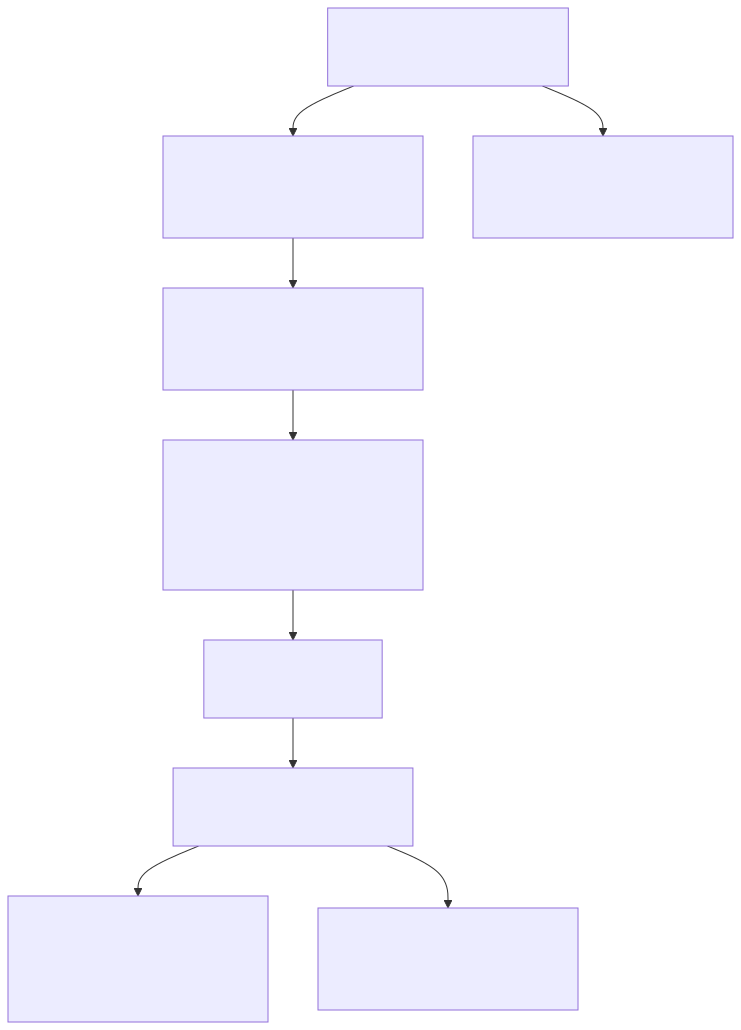
\includegraphics[width=\maxwidth,keepaspectratio,alt={Mermaid Diagram 1}]{0009-session-start-protocol/mermaid_1.png}}
\caption{Mermaid Diagram 1}
\end{figure}

\begin{longtable}[]{@{}
  >{\raggedright\arraybackslash}p{(\linewidth - 6\tabcolsep) * \real{0.1507}}
  >{\raggedright\arraybackslash}p{(\linewidth - 6\tabcolsep) * \real{0.1096}}
  >{\raggedright\arraybackslash}p{(\linewidth - 6\tabcolsep) * \real{0.3425}}
  >{\raggedright\arraybackslash}p{(\linewidth - 6\tabcolsep) * \real{0.3973}}@{}}
\toprule\noalign{}
\begin{minipage}[b]{\linewidth}\raggedright
Field
\end{minipage} & \begin{minipage}[b]{\linewidth}\raggedright
Size
\end{minipage} & \begin{minipage}[b]{\linewidth}\raggedright
Description
\end{minipage} & \begin{minipage}[b]{\linewidth}\raggedright
Value
\end{minipage} \\
\midrule\noalign{}
\endhead
\bottomrule\noalign{}
\endlastfoot
\textbf{Version} & 1 byte & Protocol version & MUST be \codebubble{0x02}
for version 2 \\
\textbf{Type} & 1 byte & Message type discriminant & See Message Types
table below \\
\textbf{Length} & 2 bytes & Payload length in bytes & 0-65535 \\
\textbf{Payload} & Variable & Message-specific data & CBOR-encoded where
applicable \\
\end{longtable}

\paragraph{4.2.1 Message Types}\label{message-types}

\begin{longtable}[]{@{}
  >{\raggedright\arraybackslash}p{(\linewidth - 4\tabcolsep) * \real{0.1471}}
  >{\raggedright\arraybackslash}p{(\linewidth - 4\tabcolsep) * \real{0.2843}}
  >{\raggedright\arraybackslash}p{(\linewidth - 4\tabcolsep) * \real{0.5686}}@{}}
\toprule\noalign{}
\begin{minipage}[b]{\linewidth}\raggedright
Type Code
\end{minipage} & \begin{minipage}[b]{\linewidth}\raggedright
Name
\end{minipage} & \begin{minipage}[b]{\linewidth}\raggedright
Description
\end{minipage} \\
\midrule\noalign{}
\endhead
\bottomrule\noalign{}
\endlastfoot
\codebubble{0x00} & StartSession & Initiates a new session \\
\codebubble{0x01} & SessionEstablished & Confirms session
establishment \\
\codebubble{0x02} & SessionError & Reports session establishment
failure \\
\codebubble{0x03} & KeepAlive & Maintains session liveness \\
\end{longtable}

\clearpage

\paragraph{4.2.2 Byte Order}\label{byte-order}

All multi-byte integer fields and values in the session start protocol
MUST be encoded and interpreted in network byte order (big-endian). This
applies to the following fields:

\textbf{Protocol message fields:}

\begin{itemize}
\tightlist
\item
  \textbf{Length} field (2 bytes) in the common message format
\item
  \textbf{Challenge} field (8 bytes) in \codebubble{StartSession},
  \codebubble{SessionEstablished}, and \\ \codebubble{SessionError}
  messages
\item
  \textbf{Additional Data} field (4 bytes) in \codebubble{StartSession}
  messages
\item
  \textbf{Additional Data} field (8 bytes) in \codebubble{KeepAlive}
  messages
\item
  \textbf{Session ID suffix} (64-bit) in HOPR session ID format (see
  Appendix 1)
\item
  Any future numeric fields added to the protocol
\end{itemize}

This requirement ensures consistent interpretation across different
architectures \\(e.g., x86, ARM, RISC-V) and prevents interoperability
issues between implementations.

\clearpage

\subsubsection{4.3 StartSession Message}\label{startsession-message}

The \codebubble{StartSession} message initiates a new session with a
remote peer. The entry node sends this message to request session
establishment, specifying the desired target endpoint and capability
flags.

\begin{figure}
\centering
\pandocbounded{\includegraphics[width=\maxwidth,keepaspectratio,alt={Mermaid Diagram 2}]{0009-session-start-protocol/mermaid_2.png}}
\caption{Mermaid Diagram 2}
\end{figure}

\begin{longtable}[]{@{}
  >{\raggedright\arraybackslash}p{(\linewidth - 6\tabcolsep) * \real{0.1275}}
  >{\raggedright\arraybackslash}p{(\linewidth - 6\tabcolsep) * \real{0.0537}}
  >{\raggedright\arraybackslash}p{(\linewidth - 6\tabcolsep) * \real{0.3490}}
  >{\raggedright\arraybackslash}p{(\linewidth - 6\tabcolsep) * \real{0.4698}}@{}}
\toprule\noalign{}
\begin{minipage}[b]{\linewidth}\raggedright
Field
\end{minipage} & \begin{minipage}[b]{\linewidth}\raggedright
Size
\end{minipage} & \begin{minipage}[b]{\linewidth}\raggedright
Description
\end{minipage} & \begin{minipage}[b]{\linewidth}\raggedright
Notes
\end{minipage} \\
\midrule\noalign{}
\endhead
\bottomrule\noalign{}
\endlastfoot
\textbf{Challenge} & 8 bytes & Random challenge for correlating
responses & MUST be generated using CSPRNG to prevent prediction \\
\textbf{Capabilities} & 1 byte & Session capabilities bitmap & See
Capability Flags table; unrecognised bits SHOULD be ignored \\
\textbf{Additional Data} & 4 bytes & Capability-dependent options & Set
to \codebubble{0x00000000} if unused; interpretation depends on
capabilities \\
\textbf{Target} & Variable & CBOR-encoded session target & Examples:
\codebubble{"127.0.0.1:1234"}, \codebubble{"wss://relay.example.com:443"} 
\end{longtable}

\clearpage

\paragraph{4.3.1 Capability Flags}\label{capability-flags}

\begin{longtable}[]{@{}
  >{\raggedright\arraybackslash}p{(\linewidth - 4\tabcolsep) * \real{0.0891}}
  >{\raggedright\arraybackslash}p{(\linewidth - 4\tabcolsep) * \real{0.2574}}
  >{\raggedright\arraybackslash}p{(\linewidth - 4\tabcolsep) * \real{0.6535}}@{}}
\toprule\noalign{}
\begin{minipage}[b]{\linewidth}\raggedright
Bit
\end{minipage} & \begin{minipage}[b]{\linewidth}\raggedright
Flag Name
\end{minipage} & \begin{minipage}[b]{\linewidth}\raggedright
Description
\end{minipage} \\
\midrule\noalign{}
\endhead
\bottomrule\noalign{}
\endlastfoot
0 & Reserved & Reserved for future use \\
1 & Reserved & Reserved for future use \\
2 & Reserved & Reserved for future use \\
3 & Reserved & Reserved for future use \\
4 & Reserved & Reserved for future use \\
5 & Reserved & Reserved for future use \\
6 & Reserved & Reserved for future use \\
7 & Reserved & Reserved for future use \\
\end{longtable}

\subsubsection{4.4 SessionEstablished Message}\label{sessionestablished-message}

The \codebubble{SessionEstablished} message confirms successful session
establishment. The exit node sends this message in response to a valid
\codebubble{StartSession} request, assigning a unique session ID that
will be used for all subsequent communication in this session.

\begin{figure}
\centering
\pandocbounded{\includegraphics[width=\maxwidth,keepaspectratio,alt={Mermaid Diagram 3}]{0009-session-start-protocol/mermaid_3.png}}
\caption{Mermaid Diagram 3}
\end{figure}

\begin{longtable}[]{@{}
  >{\raggedright\arraybackslash}p{(\linewidth - 6\tabcolsep) * \real{0.1517}}
  >{\raggedright\arraybackslash}p{(\linewidth - 6\tabcolsep) * \real{0.0552}}
  >{\raggedright\arraybackslash}p{(\linewidth - 6\tabcolsep) * \real{0.2759}}
  >{\raggedright\arraybackslash}p{(\linewidth - 6\tabcolsep) * \real{0.5172}}@{}}
\toprule\noalign{}
\begin{minipage}[b]{\linewidth}\raggedright
Field
\end{minipage} & \begin{minipage}[b]{\linewidth}\raggedright
Size
\end{minipage} & \begin{minipage}[b]{\linewidth}\raggedright
Description
\end{minipage} & \begin{minipage}[b]{\linewidth}\raggedright
Notes
\end{minipage} \\
\midrule\noalign{}
\endhead
\bottomrule\noalign{}
\endlastfoot
\textbf{Original Challenge} & 8 bytes & Challenge from
\codebubble{StartSession} message & MUST exactly match the challenge
from the initiating \codebubble{StartSession} request \\
\textbf{Session ID} & Variable & CBOR-encoded session identifier &
Assigned by exit node; MUST be unique within exit node's session
namespace \\
\end{longtable}

\clearpage

\subsubsection{4.5 SessionError Message}\label{sessionerror-message}

The \codebubble{SessionError} message reports session establishment
failure. The exit node sends this message when it cannot establish a
session, providing a specific error code to indicate the reason for
failure. This enables the entry node to implement intelligent retry
logic or select alternative exit nodes.

\begin{figure}
\centering
\pandocbounded{\includegraphics[width=\maxwidth,keepaspectratio,alt={Mermaid Diagram 4}]{0009-session-start-protocol/mermaid_4.png}}
\caption{Mermaid Diagram 4}
\end{figure}

\begin{longtable}[]{@{}
  >{\raggedright\arraybackslash}p{(\linewidth - 6\tabcolsep) * \real{0.0963}}
  >{\raggedright\arraybackslash}p{(\linewidth - 6\tabcolsep) * \real{0.0519}}
  >{\raggedright\arraybackslash}p{(\linewidth - 6\tabcolsep) * \real{0.2963}}
  >{\raggedright\arraybackslash}p{(\linewidth - 6\tabcolsep) * \real{0.5556}}@{}}
\toprule\noalign{}
\begin{minipage}[b]{\linewidth}\raggedright
Field
\end{minipage} & \begin{minipage}[b]{\linewidth}\raggedright
Size
\end{minipage} & \begin{minipage}[b]{\linewidth}\raggedright
Description
\end{minipage} & \begin{minipage}[b]{\linewidth}\raggedright
Notes
\end{minipage} \\
\midrule\noalign{}
\endhead
\bottomrule\noalign{}
\endlastfoot
\textbf{Challenge} & 8 bytes & Challenge from \codebubble{StartSession}
message & MUST exactly match the challenge from the initiating
\codebubble{StartSession} request \\
\textbf{Reason} & 1 byte & Error reason code & See Error Codes table
below \\
\end{longtable}

\clearpage

\paragraph{4.5.1 Error Codes}\label{error-codes}

\begin{longtable}[]{@{}
  >{\raggedright\arraybackslash}p{(\linewidth - 6\tabcolsep) * \real{0.0426}}
  >{\raggedright\arraybackslash}p{(\linewidth - 6\tabcolsep) * \real{0.1277}}
  >{\raggedright\arraybackslash}p{(\linewidth - 6\tabcolsep) * \real{0.3688}}
  >{\raggedright\arraybackslash}p{(\linewidth - 6\tabcolsep) * \real{0.4610}}@{}}
\toprule\noalign{}
\begin{minipage}[b]{\linewidth}\raggedright
Code
\end{minipage} & \begin{minipage}[b]{\linewidth}\raggedright
Name
\end{minipage} & \begin{minipage}[b]{\linewidth}\raggedright
Description
\end{minipage} & \begin{minipage}[b]{\linewidth}\raggedright
Recommended Action
\end{minipage} \\
\midrule\noalign{}
\endhead
\bottomrule\noalign{}
\endlastfoot
\codebubble{0x00} & Unknown Error & Unspecified error condition & Retry
with different parameters or select alternative exit node \\
\codebubble{0x01} & No Slots Available & Exit node has no available
session slots & Retry after delay or select alternative exit node \\
\codebubble{0x02} & Busy & Exit node is temporarily busy processing
requests & Retry after brief exponential backoff delay \\
\end{longtable}

\subsubsection{4.6 KeepAlive Message}\label{keepalive-message}

The \codebubble{KeepAlive} message maintains session liveness. Either
peer can send this message periodically to signal that the session is
still active and prevent session timeout. The frequency of keep-alive
messages depends on the session timeout policy of the peers.

\begin{figure}
\centering
\pandocbounded{\includegraphics[width=\maxwidth,keepaspectratio,alt={Mermaid Diagram 5}]{0009-session-start-protocol/mermaid_5.png}}
\caption{Mermaid Diagram 5}
\end{figure}

\begin{longtable}[]{@{}
  >{\raggedright\arraybackslash}p{(\linewidth - 6\tabcolsep) * \real{0.1293}}
  >{\raggedright\arraybackslash}p{(\linewidth - 6\tabcolsep) * \real{0.0544}}
  >{\raggedright\arraybackslash}p{(\linewidth - 6\tabcolsep) * \real{0.2721}}
  >{\raggedright\arraybackslash}p{(\linewidth - 6\tabcolsep) * \real{0.5442}}@{}}
\toprule\noalign{}
\begin{minipage}[b]{\linewidth}\raggedright
Field
\end{minipage} & \begin{minipage}[b]{\linewidth}\raggedright
Size
\end{minipage} & \begin{minipage}[b]{\linewidth}\raggedright
Description
\end{minipage} & \begin{minipage}[b]{\linewidth}\raggedright
Notes
\end{minipage} \\
\midrule\noalign{}
\endhead
\bottomrule\noalign{}
\endlastfoot
\textbf{Flags} & 1 byte & Reserved for future use & MUST be set to
\codebubble{0x00} by senders; SHOULD be ignored by receivers \\
\textbf{Additional Data} & 8 bytes & Flag-dependent options & Set to
\codebubble{0x0000000000000000} if unused; interpretation may depend on
future flags \\
\textbf{Session ID} & Variable & CBOR-encoded session identifier & MUST
match an established session ID \\
\end{longtable}

\subsubsection{4.7 Protocol Flow}\label{protocol-flow}

\begin{figure}
\centering
\pandocbounded{\includegraphics[width=\maxwidth,keepaspectratio,alt={Mermaid Diagram 6}]{0009-session-start-protocol/mermaid_6.png}}
\caption{Mermaid Diagram 6}
\end{figure}

\clearpage

\subsubsection{4.8 Protocol Constants}\label{protocol-constants}

\begin{longtable}[]{@{}
  >{\raggedright\arraybackslash}p{(\linewidth - 4\tabcolsep) * \real{0.2472}}
  >{\raggedright\arraybackslash}p{(\linewidth - 4\tabcolsep) * \real{0.1236}}
  >{\raggedright\arraybackslash}p{(\linewidth - 4\tabcolsep) * \real{0.6292}}@{}}
\toprule\noalign{}
\begin{minipage}[b]{\linewidth}\raggedright
Constant
\end{minipage} & \begin{minipage}[b]{\linewidth}\raggedright
Value
\end{minipage} & \begin{minipage}[b]{\linewidth}\raggedright
Description
\end{minipage} \\
\midrule\noalign{}
\endhead
\bottomrule\noalign{}
\endlastfoot
\textbf{Protocol Version} & \codebubble{0x02} & Current protocol
version \\
\textbf{Default Timeout} & 30 seconds & Default session establishment
timeout (SHOULD be configurable) \\
\textbf{Challenge Size} & 8 bytes & Fixed size for challenge field \\
\textbf{Max Payload Length} & 65535 bytes & Maximum message payload size
(limited by Length field) \\
\end{longtable}

\subsubsection{4.9 Protocol Rules}\label{protocol-rules}

\begin{longtable}[]{@{}
  >{\raggedright\arraybackslash}p{(\linewidth - 4\tabcolsep) * \real{0.1825}}
  >{\raggedright\arraybackslash}p{(\linewidth - 4\tabcolsep) * \real{0.1241}}
  >{\raggedright\arraybackslash}p{(\linewidth - 4\tabcolsep) * \real{0.6934}}@{}}
\toprule\noalign{}
\begin{minipage}[b]{\linewidth}\raggedright
Rule
\end{minipage} & \begin{minipage}[b]{\linewidth}\raggedright
Requirement Level
\end{minipage} & \begin{minipage}[b]{\linewidth}\raggedright
Description
\end{minipage} \\
\midrule\noalign{}
\endhead
\bottomrule\noalign{}
\endlastfoot
\textbf{Challenge Generation} & MUST & Challenge values MUST be randomly
generated using a cryptographically secure PRNG \\
\textbf{Session ID Uniqueness} & MUST & Session IDs MUST be unique
within the exit node's session namespace \\
\textbf{Byte Order} & MUST & All multi-byte integer fields MUST use
network byte order (big-endian) \\
\textbf{CBOR Encoding} & MUST & Session targets and session IDs MUST use
CBOR encoding {[}01{]} \\
\textbf{Payload Limits} & MUST & Messages MUST fit within HOPR packet
payload limits (see
\href{../RFC-0004-hopr-packet-protocol/0004-hopr-packet-protocol.md}{RFC-0004}) \\
\textbf{Keep-Alive Frequency} & SHOULD & \codebubble{KeepAlive} messages
SHOULD be sent periodically to maintain long-lived sessions \\
\textbf{Error Handling} & MUST & Implementations MUST handle all defined
error conditions gracefully \\
\textbf{Timeout Configuration} & SHOULD & Session establishment timeouts
SHOULD be configurable (default: 30s) \\
\end{longtable}

\clearpage

\subsubsection{4.10 Example Message
Exchanges}\label{example-message-exchanges}

\paragraph{4.10.1 Successful Session
Establishment}\label{successful-session-establishment}

Complete successful session establishment with immediate keep-alive:

\begin{figure}
\centering
\pandocbounded{\includegraphics[width=\maxwidth,keepaspectratio,alt={Mermaid Diagram 7}]{0009-session-start-protocol/mermaid_7.png}}
\caption{Mermaid Diagram 7}
\end{figure}

\paragraph{4.10.2 Session Establishment
Failure}\label{session-establishment-failure}

Session establishment failing due to resource exhaustion:

\begin{figure}
\centering
\pandocbounded{\includegraphics[width=\maxwidth,keepaspectratio,alt={Mermaid Diagram 8}]{0009-session-start-protocol/mermaid_8.png}}
\caption{Mermaid Diagram 8}
\end{figure}

\clearpage

\paragraph{4.10.3 Session Establishment
Timeout}\label{session-establishment-timeout}

Session establishment with no response from exit node, resulting in
timeout:

\begin{figure}
\centering
\pandocbounded{\includegraphics[width=\maxwidth,keepaspectratio,alt={Mermaid Diagram 9}]{0009-session-start-protocol/mermaid_9.png}}
\caption{Mermaid Diagram 9}
\end{figure}

\paragraph{4.10.4 Long-Running Session with Periodic
Keep-Alives}\label{long-running-session-with-periodic-keep-alives}

Maintaining an established session over time:

\begin{figure}
\centering
\pandocbounded{\includegraphics[width=\maxwidth,keepaspectratio,alt={Mermaid Diagram 10}]{0009-session-start-protocol/mermaid_10.png}}
\caption{Mermaid Diagram 10}
\end{figure}

\subsection{5. Design Considerations}\label{design-considerations}

\subsubsection{5.1 CBOR Encoding}\label{cbor-encoding}

The use of CBOR (Concise Binary Object Representation) {[}01{]} for
session IDs and session targets provides several advantages:

\begin{itemize}
\tightlist
\item
  \textbf{Flexible data types}: Supports various data types without
  fixed-size constraints, enabling session IDs and targets to be
  represented as integers, strings, byte arrays, or structured data.
\item
  \textbf{Compact binary encoding}: More efficient than text-based
  formats like JSON, reducing packet overhead in the constrained HOPR
  packet payload.
\item
  \textbf{Language-agnostic serialisation}: Standardised format with
  implementations available in multiple programming languages,
  facilitating interoperability.
\item
  \textbf{Support for complex identifiers}: Enables session identifiers
  to encode additional metadata when needed (e.g., node identifiers,
  timestamps, or routing hints).
\end{itemize}

\subsubsection{5.2 Challenge-Response
Design}\label{challenge-response-design}

The 64-bit challenge field serves multiple purposes in the session start
protocol:

\begin{itemize}
\tightlist
\item
  \textbf{Request-response correlation}: Enables the entry node to match
  \codebubble{SessionEstablished} or \codebubble{SessionError} responses
  to the corresponding \codebubble{StartSession} request, even when
  multiple requests are pending simultaneously.
\item
  \textbf{Protection against replay attacks}: When combined with
  transport-level security, the unpredictable challenge prevents an
  attacker from replaying a captured \codebubble{StartSession} message
  to establish unauthorised sessions.
\item
  \textbf{Simple state tracking}: The challenge allows implementations
  to maintain minimal state for pending session establishment requests,
  using the challenge as a key in a hash table or similar data
  structure.
\item
  \textbf{Low collision probability}: With 2\^{}64 possible values and
  cryptographically secure random generation, the probability of
  challenge collisions is negligible even with many concurrent requests.
\end{itemize}

\subsubsection{5.3 Capability Negotiation}\label{capability-negotiation}

The single-byte capability field provides a compact mechanism for
protocol negotiation:

\begin{itemize}
\tightlist
\item
  \textbf{Up to 8 independent flags}: Each bit can represent a distinct
  capability, allowing peers to negotiate multiple features
  simultaneously.
\item
  \textbf{Future protocol extensions}: As new session features are
  developed, capability bits can be assigned without changing the
  message format or breaking existing implementations.
\item
  \textbf{Backward compatibility}: Implementations can safely ignore
  unrecognised capability bits, allowing newer implementations to
  interoperate with older ones that don't support new features.
\item
  \textbf{Minimal overhead}: A single byte adds negligible overhead
  while providing sufficient flexibility for anticipated protocol
  evolution.
\end{itemize}

\subsubsection{5.4 Transport Independence}\label{transport-independence}

The session start protocol is intentionally transport-agnostic, making
it suitable for various network environments:

\begin{itemize}
\tightlist
\item
  \textbf{Packet-based transport}: Works over any packet-based transport
  layer that provides bidirectional communication.
\item
  \textbf{Designed for HOPR, not limited to it}: While optimised for
  HOPR packets
  (\href{../RFC-0004-hopr-packet-protocol/0004-hopr-packet-protocol.md}{RFC-0004}),
  the protocol can be used over other transports such as raw UDP,
  WebSockets, or QUIC.
\item
  \textbf{No ordering assumptions}: The protocol does not require
  ordered message delivery, making it suitable for unreliable
  transports.
\item
  \textbf{No reliability assumptions}: The protocol does not depend on
  reliable delivery; implementations can add timeouts and retransmission
  logic as needed for their specific transport.
\end{itemize}

\subsubsection{5.5 Error Handling}\label{error-handling}

The protocol provides structured error reporting to enable intelligent
failure handling:

\begin{itemize}
\tightlist
\item
  \textbf{Specific error codes}: Well-defined error codes (Unknown
  Error, No Slots Available, Busy) enable entry nodes to distinguish
  between different failure scenarios and adjust their behaviour
  accordingly.
\item
  \textbf{Challenge correlation}: Including the original challenge in
  error messages ensures that entry nodes can correctly attribute errors
  to specific requests.
\item
  \textbf{Graceful resource exhaustion}: The ``No Slots Available''
  error allows exit nodes to signal capacity limits without dropping
  requests silently, enabling entry nodes to try alternative exit nodes.
\item
  \textbf{Temporary vs.~permanent failures}: The error code taxonomy
  distinguishes between temporary failures (Busy) that warrant retry and
  semi-permanent failures (No Slots Available) that suggest trying a
  different node.
\end{itemize}

\subsection{6. Compatibility}\label{compatibility}

\subsubsection{6.1 Version Compatibility}\label{version-compatibility}

\begin{itemize}
\tightlist
\item
  Version 2 (\codebubble{0x02}) is the initial version of the session
  start protocol specified in this document.
\item
  Future versions MUST use different version numbers to distinguish
  themselves from version 2.
\item
  Implementations MUST reject messages with unknown or unsupported
  version numbers.
\item
  Version negotiation mechanisms are out of scope for this
  specification; if needed, they should be addressed in future RFCs.
\end{itemize}

\subsubsection{6.2 Transport Requirements}\label{transport-requirements}

\begin{itemize}
\tightlist
\item
  The protocol requires a bidirectional communication channel between
  entry and exit nodes.
\item
  No assumptions are made about message ordering; messages may arrive
  out of order.
\item
  No assumptions are made about reliability; implementations should add
  timeout and retransmission logic as appropriate.
\item
  Compatible with any transport that provides packet delivery (e.g.,
  UDP, HOPR packets, QUIC, WebSockets).
\item
  Designed for the HOPR mixnet but not limited to it; the protocol can
  be deployed over other privacy-preserving or traditional networks.
\end{itemize}

\subsubsection{6.3 Integration with HOPR Session Data
Protocol}\label{integration-with-hopr-session-data-protocol}

\begin{itemize}
\tightlist
\item
  The session start protocol establishes sessions that are subsequently
  used by the session data protocol
  (\href{../RFC-0008-session-protocol/0008-session-protocol.md}{RFC-0008})
  for reliable and unreliable data transmission.
\item
  Session IDs assigned by this protocol are used to identify data
  sessions in the session data protocol.
\item
  The two protocols operate independently: session start handles
  handshake and lifecycle, while session data handles message
  transmission.
\item
  Session establishment MUST complete successfully before data
  transmission can begin.
\end{itemize}

\subsection{7. Security Considerations}\label{security-considerations}

\subsubsection{7.1 Protocol Security}\label{protocol-security}

\begin{itemize}
\tightlist
\item
  The session start protocol provides NO encryption or authentication by
  itself.
\item
  Security properties (confidentiality, integrity, authenticity) MUST be
  provided by the underlying transport layer.
\item
  Session IDs SHOULD be unpredictable to prevent session hijacking and
  enumeration attacks.
\item
  Challenges MUST be generated using cryptographically secure random
  number generation to prevent prediction and replay attacks.
\end{itemize}

\subsubsection{7.2 Attack Vectors}\label{attack-vectors}

The following attack vectors exist when the protocol is used without
adequate transport-level security:

\begin{itemize}
\tightlist
\item
  \textbf{Replay attacks}: Captured \codebubble{StartSession} messages
  can be replayed without additional timestamp or nonce mechanisms.
  Mitigation requires transport-level encryption and authentication.
\item
  \textbf{Man-in-the-middle attacks}: The protocol alone does not
  prevent an active attacker from intercepting and modifying messages.
  Transport-level security is required.
\item
  \textbf{Information disclosure}: Session targets may expose service
  information \\(e.g., destination addresses) if not encrypted at the
  transport layer.
\item
  \textbf{Resource exhaustion}: Attackers can flood exit nodes with
  excessive session establishment requests, potentially exhausting
  available session slots. Rate limiting is essential.
\item
  \textbf{Session hijacking}: Predictable session IDs enable attackers
  to guess valid session identifiers and hijack established sessions.
  Session IDs MUST be generated unpredictably.
\end{itemize}

\clearpage

\subsubsection{7.3 Mitigation Strategies}\label{mitigation-strategies}

Implementations SHOULD employ the following strategies to mitigate
security risks:

\begin{itemize}
\tightlist
\item
  \textbf{Transport-level security}: Use HOPR packet encryption
  (\href{../RFC-0004-hopr-packet-protocol/0004-hopr-packet-protocol.md}{RFC-0004})
  or other transport-level encryption and authentication mechanisms to
  protect against replay, man-in-the-middle, and information disclosure
  attacks.
\item
  \textbf{Rate limiting}: Implement rate limiting for incoming session
  establishment requests to prevent resource exhaustion attacks. Limits
  can be per-peer or global.
\item
  \textbf{Unpredictable session identifiers}: Generate session IDs using
  cryptographically secure random number generators to prevent session
  hijacking and enumeration.
\item
  \textbf{Session timeout mechanisms}: Implement session timeouts to
  automatically clean up stale sessions and free resources. Keep-alive
  messages can be used to maintain active sessions.
\item
  \textbf{Challenge expiration}: Optionally expire challenges after a
  configurable timeout to limit the window for replay attacks.
\end{itemize}

\subsection{8. Future Work}\label{future-work}

Potential areas for future protocol enhancements include:

\begin{itemize}
\tightlist
\item
  \textbf{Session parameter renegotiation}: Mechanisms to renegotiate
  session parameters (capabilities, targets) without tearing down and
  re-establishing the session.
\item
  \textbf{Performance optimisations}: Techniques to reduce session
  establishment latency for high-frequency session creation scenarios,
  such as session pooling or 0-RTT establishment.
\item
  \textbf{Enhanced capability negotiation}: More sophisticated
  capability negotiation mechanisms, including capability versioning and
  feature discovery.
\item
  \textbf{Heartbeat and health monitoring}: Enhanced keep-alive
  mechanisms that can carry health status information or
  quality-of-service metrics.
\end{itemize}

\clearpage

\subsection{9. Implementation Notes}\label{implementation-notes}

\subsubsection{9.1 Testing
Recommendations}\label{testing-recommendations}

Implementations SHOULD include comprehensive tests covering:

\begin{itemize}
\tightlist
\item
  \textbf{Session target format variations}: Test with various session
  target formats (IPv4, IPv6, service URIs, edge cases) to ensure
  correct CBOR encoding and decoding.
\item
  \textbf{Network failure simulation}: Simulate packet loss, delays, and
  timeouts to verify correct timeout handling and retransmission logic.
\item
  \textbf{Challenge uniqueness and correlation}: Verify that challenges
  are generated uniquely and that responses are correctly correlated
  with requests, including handling of duplicate challenges.
\item
  \textbf{Capability negotiation edge cases}: Test capability
  negotiation with various combinations of set and unset capability
  bits, including forward and backward compatibility scenarios.
\item
  \textbf{CBOR encoding correctness}: Validate that CBOR encoding and
  decoding of session IDs and targets is correct and handles all
  expected data types.
\item
  \textbf{Error handling}: Test all error codes and verify that error
  messages are correctly generated and handled.
\end{itemize}

\subsection{10. Appendix 1}\label{appendix-1}

Within the HOPR protocol, a session is identified uniquely via the HOPR
session ID. This consists of 10 pseudo-random bytes as a prefix and a
64-bit unsigned integer as a suffix. The 64-bit suffix is encoded and
interpreted as a big-endian unsigned integer.

In human-readable format, a HOPR session ID has the following syntax:

\codebubble{0xabcdefabcdefabcdefab:123456}

The prefix (\codebubble{0xabcdefabcdefabcdefab}) represents a fixed
pseudonym prefix in the HOPR packet protocol (as specified in
\href{../RFC-0004-hopr-packet-protocol/0004-hopr-packet-protocol.md}{RFC-0004}).
The suffix (\codebubble{123456}) represents an application tag that
identifies sessions within the reserved range in the application
protocol
(\href{../RFC-0011-application-protocol/0011-application-protocol.md}{RFC-0011}).

\subsection{11. References}\label{references}

{[}01{]} Bradner, S. (1997).
{Key words for use in RFCs to Indicate Requirement Levels}. \\ \emph{IETF RFC 2119}.
\href{https://datatracker.ietf.org/doc/html/rfc2119}{\underline{https://datatracker.ietf.org/doc/html/rfc2119}}

{[}02{]} Bormann, C. \& Hoffman, P. (2013).
{Concise Binary Object Representation (CBOR)}. \emph{IETF RFC 7049}.
\href{https://datatracker.ietf.org/doc/html/rfc7049}{\underline{https://datatracker.ietf.org/doc/html/rfc7049}}